La pila presente en la placa madre de una computadora, comúnmente del tipo CR2032 \cite{profesionalpila}, desempeña un papel crucial en el mantenimiento de la configuración del sistema. Esencialmente, esta pila suministra energía constante al chip CMOS (Complementary Metal-Oxide-Semiconductor), lo que permite que se conserven ajustes vitales incluso cuando la computadora está apagada.

\begin{figure}
  \centering
  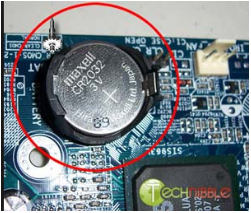
\includegraphics[scale=0.9]{imagenes/pila-cr2032.png}
  \caption{Pila CR2032}
\end{figure}

\subsubsection{Computadoras Antiguas vs. Modernas: El Rol Evolutivo de la Pila CMOS}

\textbf{Computadoras Antiguas:}

En las PCs más antiguas, la pila CMOS alimentaba directamente la CMOS RAM, una memoria de baja potencia que almacenaba la configuración del BIOS. Esto incluía ajustes de hardware, orden de arranque y la hora del sistema. Sin la pila, toda esta información se perdía al apagar la computadora \cite{profesionalpila}.

\begin{figure}
  \centering
  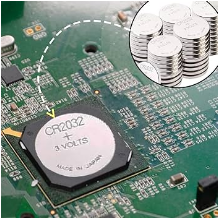
\includegraphics[scale=0.9]{imagenes/pila-cmos.png}
  \caption{Pila CMOS}
\end{figure}

En estos sistemas, la pila era indispensable para el funcionamiento básico del equipo, ya que la pérdida de la configuración del BIOS podía impedir el arranque.

\textbf{Computadoras Modernas:}

Las PCs modernas han evolucionado. Ahora, la configuración del BIOS/UEFI (Unified Extensible Firmware Interface) se almacena generalmente en memoria flash no volátil. Esto significa que la configuración se conserva incluso sin energía de la pila.

\begin{figure}
  \centering
  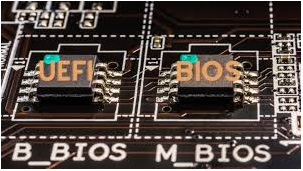
\includegraphics[scale=0.9]{imagenes/uefi-bios.png}
  \caption{Configuración BIOS/UEFI}
\end{figure}

Sin embargo, la pila CR2032 aún cumple una función esencial: alimentar el reloj de tiempo real (RTC). El RTC es un circuito independiente que mantiene la hora del sistema, independientemente de si la computadora está encendida o apagada.

\begin{figure}
  \centering
  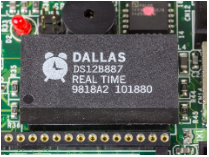
\includegraphics{imagenes/reloj.png}
  \caption{Reloj de tiempo real (RTC)}
\end{figure}

Por lo tanto, en las PCs modernas, la pila garantiza que la hora del sistema sea precisa, lo cual es vital para diversas funciones, como la programación de tareas, el registro de eventos y la sincronización de redes.

\subsubsection{Puntos Clave}

\begin{itemize}
  \item \textbf{No recargable:} Es importante destacar que la pila CR2032 no es recargable. La placa madre está diseñada con circuitos que previenen la carga y descarga de esta pila durante el funcionamiento de la computadora. Intentar recargarla podría ser peligroso \cite{pcworldpila}.
  \item \textbf{Variabilidad en la duración:} La vida útil de estas pilas puede variar, generalmente entre 3 y 5 años, aunque algunos modelos de mayor calidad pueden durar más. La duración depende de factores como la calidad de la pila y las condiciones ambientales.
  \item \textbf{Consecuencias de la falla:} Cuando la pila se agota, se pueden presentar problemas como la pérdida de la fecha y hora del sistema, el restablecimiento de la configuración del BIOS a los valores predeterminados y, en algunos casos, dificultades en el arranque de la computadora, es posible que no se pueda conectar a Internet por fecha y hora erróneas, se escucha un pitido constante \cite{vasycpila} .
\end{itemize}
